\documentclass[ignorenonframetext,aspectratio=169]{beamer}
\setbeamertemplate{caption}[numbered]
\setbeamertemplate{caption label separator}{: }
\setbeamercolor{caption name}{fg=normal text.fg}
\beamertemplatenavigationsymbolsempty
\usepackage{lmodern}
\usepackage{amssymb,amsmath}
\usepackage{ifxetex,ifluatex}
\usepackage{fixltx2e} % provides \textsubscript
\ifnum 0\ifxetex 1\fi\ifluatex 1\fi=0 % if pdftex
  \usepackage[T1]{fontenc}
  \usepackage[utf8]{inputenc}
\else % if luatex or xelatex
  \ifxetex
    \usepackage{mathspec}
  \else
    \usepackage{fontspec}
  \fi
  \defaultfontfeatures{Ligatures=TeX,Scale=MatchLowercase}
\fi
% use upquote if available, for straight quotes in verbatim environments
\IfFileExists{upquote.sty}{\usepackage{upquote}}{}
% use microtype if available
\IfFileExists{microtype.sty}{%
\usepackage{microtype}
\UseMicrotypeSet[protrusion]{basicmath} % disable protrusion for tt fonts
}{}
\newif\ifbibliography
\hypersetup{
            pdfborder={0 0 0},
            breaklinks=true}

%\DeclareUnicodeCharacter{2200}{$\forall$}
%\DeclareUnicodeCharacter{2228}{$\vee$}
%\DeclareUnicodeCharacter{2227}{$\wedge$}
%\DeclareUnicodeCharacter{00A0}{~}

\usepackage{alltt}
\usepackage{color}
\usepackage{fancyvrb}
\newcommand{\VerbBar}{|}
\newcommand{\VERB}{\Verb[commandchars=\\\{\}]}
\DefineVerbatimEnvironment{Highlighting}{Verbatim}{commandchars=\\\{\}}
% Add ',fontsize=\small' for more characters per line
\newenvironment{Shaded}{}{}
\newcommand{\KeywordTok}[1]{\textcolor[rgb]{0.00,0.44,0.13}{\textbf{{#1}}}}
\newcommand{\DataTypeTok}[1]{\textcolor[rgb]{0.56,0.13,0.00}{{#1}}}
\newcommand{\DecValTok}[1]{\textcolor[rgb]{0.25,0.63,0.44}{{#1}}}
\newcommand{\BaseNTok}[1]{\textcolor[rgb]{0.25,0.63,0.44}{{#1}}}
\newcommand{\FloatTok}[1]{\textcolor[rgb]{0.25,0.63,0.44}{{#1}}}
\newcommand{\ConstantTok}[1]{\textcolor[rgb]{0.53,0.00,0.00}{{#1}}}
\newcommand{\CharTok}[1]{\textcolor[rgb]{0.25,0.44,0.63}{{#1}}}
\newcommand{\SpecialCharTok}[1]{\textcolor[rgb]{0.25,0.44,0.63}{{#1}}}
\newcommand{\StringTok}[1]{\textcolor[rgb]{0.25,0.44,0.63}{{#1}}}
\newcommand{\VerbatimStringTok}[1]{\textcolor[rgb]{0.25,0.44,0.63}{{#1}}}
\newcommand{\SpecialStringTok}[1]{\textcolor[rgb]{0.73,0.40,0.53}{{#1}}}
\newcommand{\ImportTok}[1]{{#1}}
\newcommand{\CommentTok}[1]{\textcolor[rgb]{0.38,0.63,0.69}{\textit{{#1}}}}
\newcommand{\DocumentationTok}[1]{\textcolor[rgb]{0.73,0.13,0.13}{\textit{{#1}}}}
\newcommand{\AnnotationTok}[1]{\textcolor[rgb]{0.38,0.63,0.69}{\textbf{\textit{{#1}}}}}
\newcommand{\CommentVarTok}[1]{\textcolor[rgb]{0.38,0.63,0.69}{\textbf{\textit{{#1}}}}}
\newcommand{\OtherTok}[1]{\textcolor[rgb]{0.00,0.44,0.13}{{#1}}}
\newcommand{\FunctionTok}[1]{\textcolor[rgb]{0.02,0.16,0.49}{{#1}}}
\newcommand{\VariableTok}[1]{\textcolor[rgb]{0.10,0.09,0.49}{{#1}}}
\newcommand{\ControlFlowTok}[1]{\textcolor[rgb]{0.00,0.44,0.13}{\textbf{{#1}}}}
\newcommand{\OperatorTok}[1]{\textcolor[rgb]{0.40,0.40,0.40}{{#1}}}
\newcommand{\BuiltInTok}[1]{{#1}}
\newcommand{\ExtensionTok}[1]{{#1}}
\newcommand{\PreprocessorTok}[1]{\textcolor[rgb]{0.74,0.48,0.00}{{#1}}}
\newcommand{\AttributeTok}[1]{\textcolor[rgb]{0.49,0.56,0.16}{{#1}}}
\newcommand{\RegionMarkerTok}[1]{{#1}}
\newcommand{\InformationTok}[1]{\textcolor[rgb]{0.38,0.63,0.69}{\textbf{\textit{{#1}}}}}
\newcommand{\WarningTok}[1]{\textcolor[rgb]{0.38,0.63,0.69}{\textbf{\textit{{#1}}}}}
\newcommand{\AlertTok}[1]{\textcolor[rgb]{1.00,0.00,0.00}{\textbf{{#1}}}}
\newcommand{\ErrorTok}[1]{\textcolor[rgb]{1.00,0.00,0.00}{\textbf{{#1}}}}
\newcommand{\NormalTok}[1]{{#1}}

% Prevent slide breaks in the middle of a paragraph:
\widowpenalties 1 10000
\raggedbottom

\AtBeginPart{
  \let\insertpartnumber\relax
  \let\partname\relax
  \frame{\partpage}
}
\AtBeginSection{
  \ifbibliography
  \else
    \let\insertsectionnumber\relax
    \let\sectionname\relax
    \frame{\sectionpage}
  \fi
}
\AtBeginSubsection{
  \let\insertsubsectionnumber\relax
  \let\subsectionname\relax
  \frame{\subsectionpage}
}

\setlength{\parindent}{0pt}
\setlength{\parskip}{6pt plus 2pt minus 1pt}
\setlength{\emergencystretch}{3em}  % prevent overfull lines
\providecommand{\tightlist}{%
  \setlength{\itemsep}{0pt}\setlength{\parskip}{0pt}}
\setcounter{secnumdepth}{0}
\usefonttheme[onlymath]{serif}
\setbeamercolor{footnote mark}{fg=gray}
\setbeamerfont{footnote}{size=\tiny}
\hypersetup{colorlinks,linkcolor=,urlcolor=purple}
\usepackage[normalem]{ulem}
\usepackage{listings}
\lstset{
    basicstyle=\ttfamily\large,
    keywordstyle=\color{blue}\bfseries,
    commentstyle=\color[rgb]{0,0.5,0}\bfseries\em
}

\title{\textbf{On naming things}}
%\subtitle{}
\author{Fraser Tweedale\\\texttt{@hackuador}}
\date{August 5, 2017\\{\tt \#pyconau}}
%\institute{\input{Logo_RH_RGB_Default-ARTIFACT.pdf_tex}}

%\logo{\def\svgwidth{1.2cm} \input{Logo_RH_RGB_Default-ARTIFACT.pdf_tex}}

\begin{document}

\frame[plain]{\titlepage}

\section{Naming things is difficult}

\section{Comprehending names of things can be difficult}

\section{I'm here to help}

\part{Avoid {\em things}}

\begin{frame}[plain]
\centering
\makebox[\textwidth][c]{
\includegraphics[width=\paperwidth,height=\paperheight,keepaspectratio]{agent.jpg}}
\end{frame}

\begin{frame}[fragile]
\begin{lstlisting}[language=Python]
def num_occ(x, list_of_list_of_x):
    return [
        len([y for y in l if y == x])
        for l in list_of_list_of_x
    ]

print num_occ('b', ["aa", "ab", "ba", "bb"])
# [0, 1, 1, 2]
\end{lstlisting}
\end{frame}

\begin{frame}[fragile]
\begin{lstlisting}[language=Python]
num_occ = lambda x, list_of_list_of_x: (
    map(lambda l: len(filter(lambda y: y == x, l)),
        list_of_list_of_x)
    )
\end{lstlisting}
\end{frame}

\begin{frame}[fragile]
\begin{lstlisting}[language=Python]
eq = lambda x: lambda y: x == y

curry = lambda f: lambda a: lambda b: f(a, b)

compose = lambda g: lambda f: lambda x: g(f(x))
\end{lstlisting}
\end{frame}

\begin{frame}[fragile]
\begin{lstlisting}[language=Python]
num_occ = ( compose
    ( compose (curry(map)) (compose(len)) )
    ( compose (curry(filter)) (eq) )
)

print num_occ('b')(["aa", "ab", "ba", "bb"])
# [0, 1, 1, 2]
\end{lstlisting}
\end{frame}

\begin{frame}[plain]
\centering
\makebox[\textwidth][c]{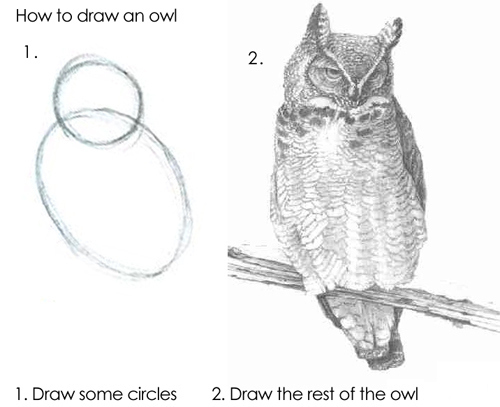
\includegraphics[width=\paperwidth,height=\paperheight,keepaspectratio]{how-to-draw-an-owl.jpg}}
\end{frame}

\begin{frame}[plain]
\centering
\makebox[\textwidth][c]{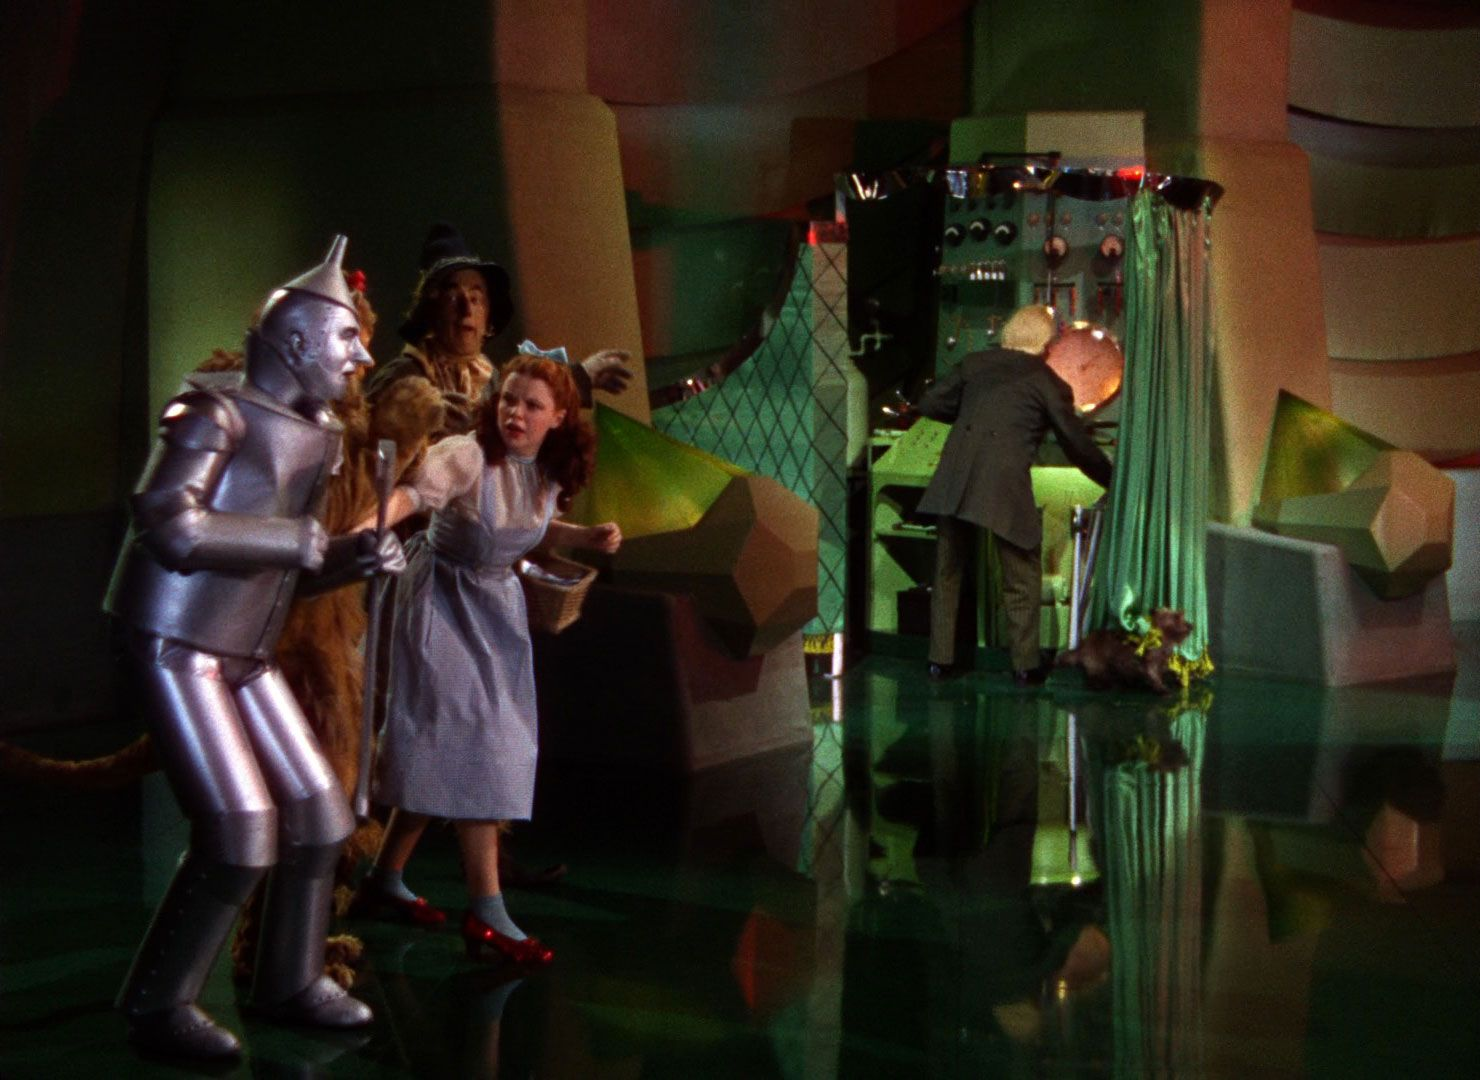
\includegraphics[width=\paperwidth,height=\paperheight,keepaspectratio]{curtain.jpg}}
\end{frame}

\begin{frame}[plain]
\centering
\makebox[\textwidth][c]{
\includegraphics[width=\paperwidth,height=\paperheight,keepaspectratio]{parens.jpg}}
\end{frame}

\part{Keep things general}

\begin{frame}[fragile]
\begin{lstlisting}[language=Python]
def identity(a):
    return a
\end{lstlisting}
\end{frame}


\part{The name is a lie}

\begin{frame}[fragile]
\begin{lstlisting}[language=Python]




def f(xs)




    return REDACTED
\end{lstlisting}
\end{frame}

\begin{frame}[fragile]
\begin{lstlisting}[language=Python]
# such PEP 484
from typing import TypeVar, List
A = TypeVar('A')

def f(xs : List[A]) -> List[A]:     # very type
    '''
            wow

    '''
    return REDACTED



\end{lstlisting}
\end{frame}

\begin{frame}[fragile]
\begin{lstlisting}[language=Python]

from typing import TypeVar, List
A = TypeVar('A')

def f(xs : List[A]) -> List[A]:
    '''
    forall x.     f([x])     = [x]
    forall xs ys. f(xs + ys) = f(ys) + f(xs)
    '''
    return REDACTED
\end{lstlisting}
\end{frame}

\begin{frame}[fragile]
\begin{lstlisting}[language=Python]

from typing import TypeVar, List
A = TypeVar('A')

def not_reverse(xs : List[A]) -> List[A]:
    '''
    forall x.     f([x])     = [x]
    forall xs ys. f(xs + ys) = f(ys) + f(xs)
    '''
    return REDACTED
\end{lstlisting}
\end{frame}


\part{Names are just labels for concepts}

\begin{frame}{A concept (abstraction)}
\begin{itemize}
\item a binary operator in some set
\item the result is always defined
\item the operator is associative
\end{itemize}
\end{frame}

\begin{frame}[fragile]
\begin{lstlisting}[language=Java]
interface IAssociativeClosedCombinable {
    ...
}




 
\end{lstlisting}
\end{frame}

\begin{frame}[fragile]
\begin{lstlisting}[language=Java]
interface IAssociativeClosedCombinable {
    ...
}

interface IAssociativeClosedCombinableWithNeutralElement
        extends IAssociativeClosedCombinable {
    ...
}
\end{lstlisting}
\end{frame}

\begin{frame}{The most useful table on Wikipedia\ldots}
\centering
\makebox[\textwidth][c]{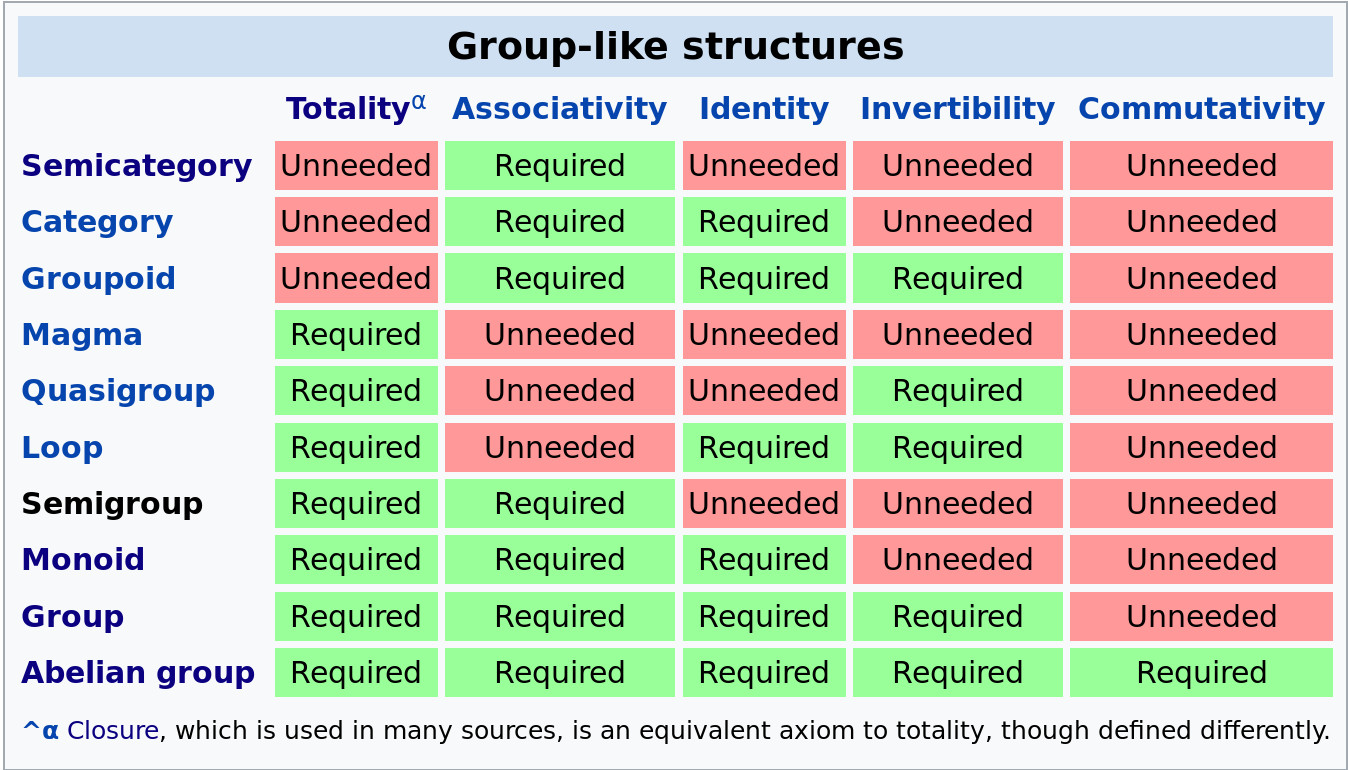
\includegraphics[width=\textwidth,height=0.8\textheight,keepaspectratio]{algebra.jpg}}
\tiny \url{https://en.wikipedia.org/wiki/Template:Group-like_structures}
\end{frame}

\begin{frame}[plain]
\centering
\makebox[\textwidth][c]{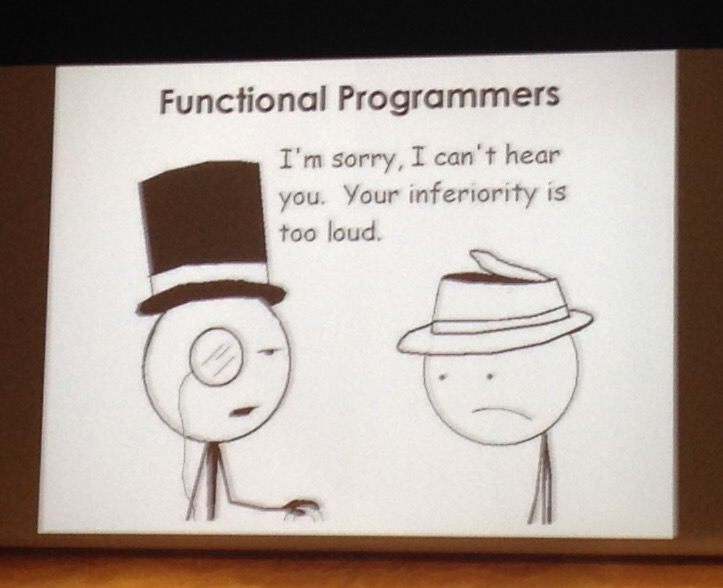
\includegraphics[width=\textwidth,height=\pageheight,keepaspectratio]{inferiority.jpg}}
\end{frame}

\begin{frame}[plain]
\centering
\makebox[\textwidth][c]{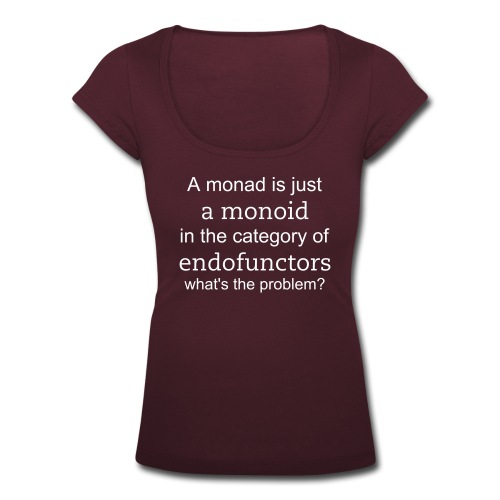
\includegraphics[width=\textwidth,height=\pageheight,keepaspectratio]{monad-shirt.jpg}}
\end{frame}


\begin{frame}[plain]

\begin{columns}

  \begin{column}{.3\textwidth}
    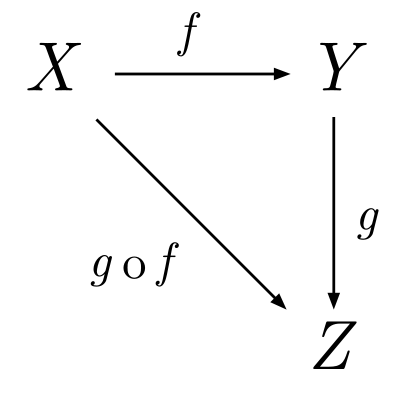
\includegraphics[width=\textwidth]{commutative-diagram.png}
  \end{column}

  \begin{column}{.7\textwidth}

    \setlength{\parskip}{.5em}

    { \centering

    \input{cc-by-ARTIFACT.pdf_tex}
    \\
    { \scriptsize
    Except where otherwise noted this work is licensed under
    }\\
    { \footnotesize
    \textbf{http://creativecommons.org/licenses/by/4.0/}
    }

    \bigskip

    \large \url{https://speakerdeck.com/frasertweedale}

    \texttt{@hackuador}

    }
  \end{column}

\end{columns}

\end{frame}

\end{document}
